\documentclass[UTF8]{ctexart}
\usepackage{geometry}
\usepackage{graphicx}
\usepackage[namelimits]{amsmath} %数学公式
\usepackage{amssymb}             %数学公式             %数学字体
\usepackage{mathrsfs} 
\usepackage{txfonts}
\usepackage{float}  %设置图片浮动位置的宏包
\usepackage{subfigure}%插入多图时用子图显示的宏包
\geometry{a4paper,scale=0.80}
\author{左熙辰-2000012103}
\date{}
\title{植物学实验1}
\ctexset{
    section/name= {实验操作}
}
\begin{document}
    \maketitle
    \section{水绵、海带的形态、结构与生殖}
        \subsection*{结果}
            \paragraph*{1.用简图或照片显示水绵的细胞形态,标注出细胞壁、细胞核、载色体及蛋白核等:}
            \begin{figure}[h]
                \centering
                \subfigure[水绵显微照片]{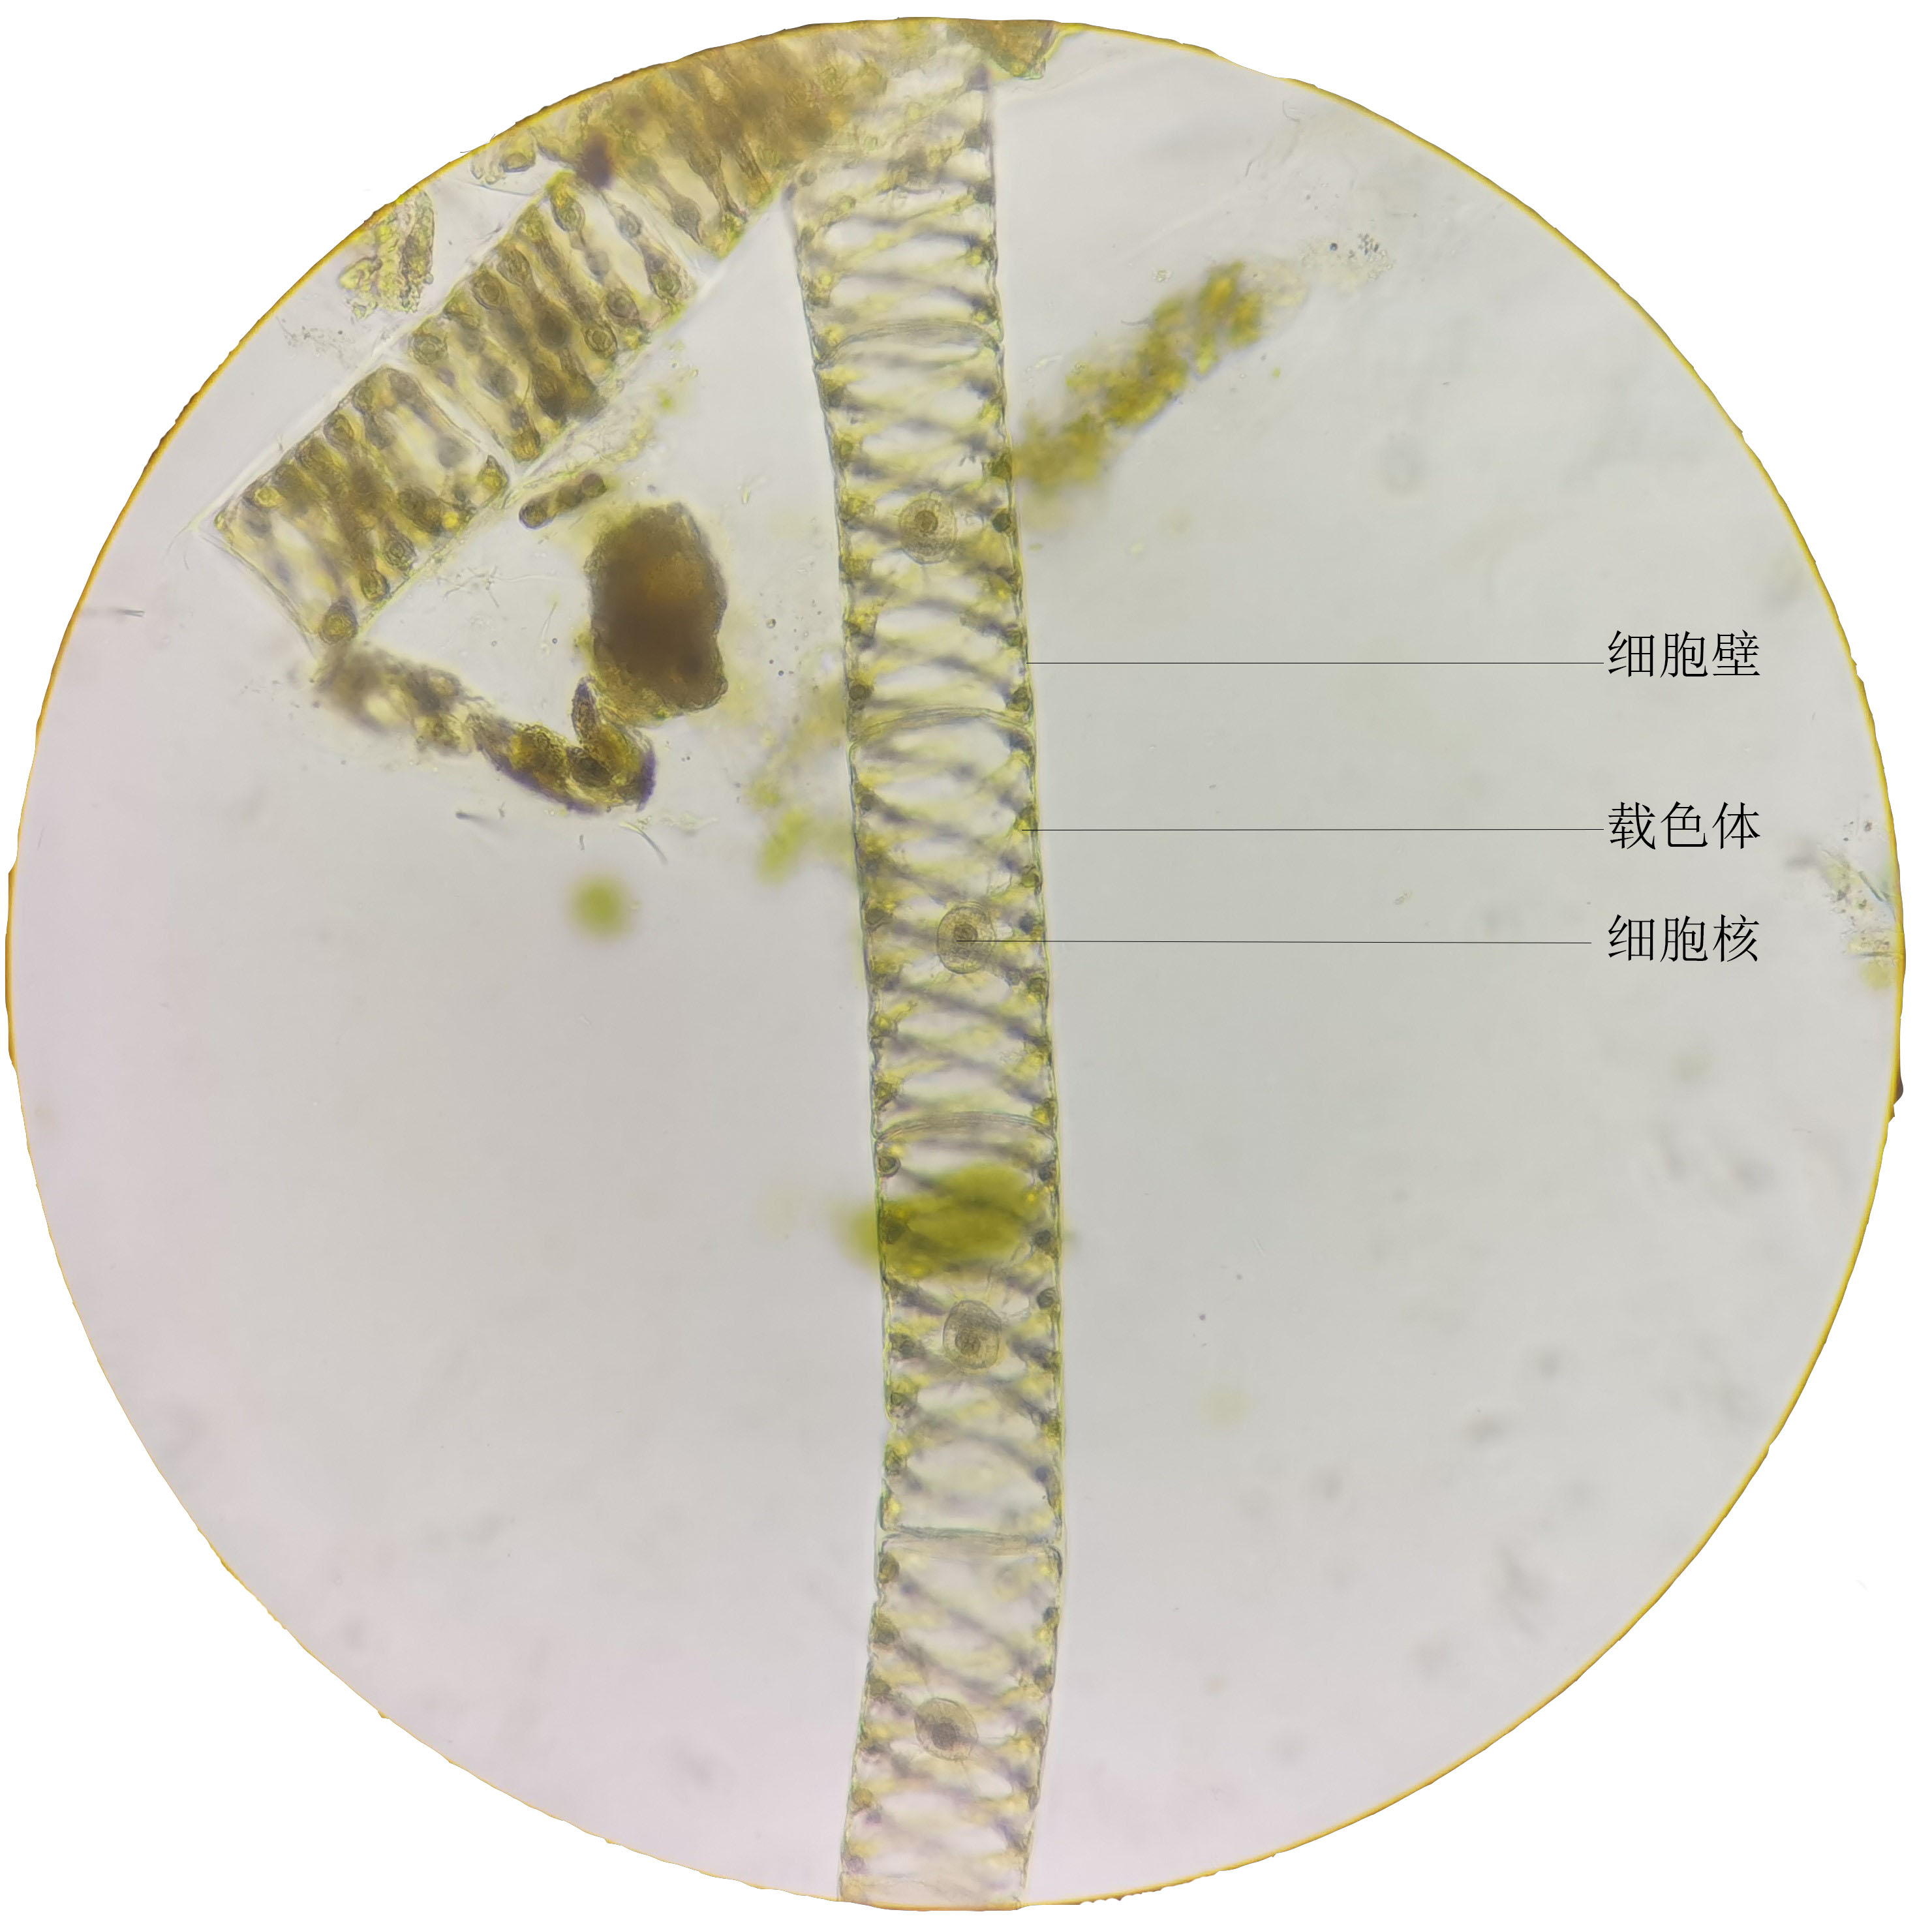
\includegraphics[scale = 0.1]{src/botany/IMG_20201118_192927.jpg}\label{shuimian}}
                \subfigure[海带带片细胞]{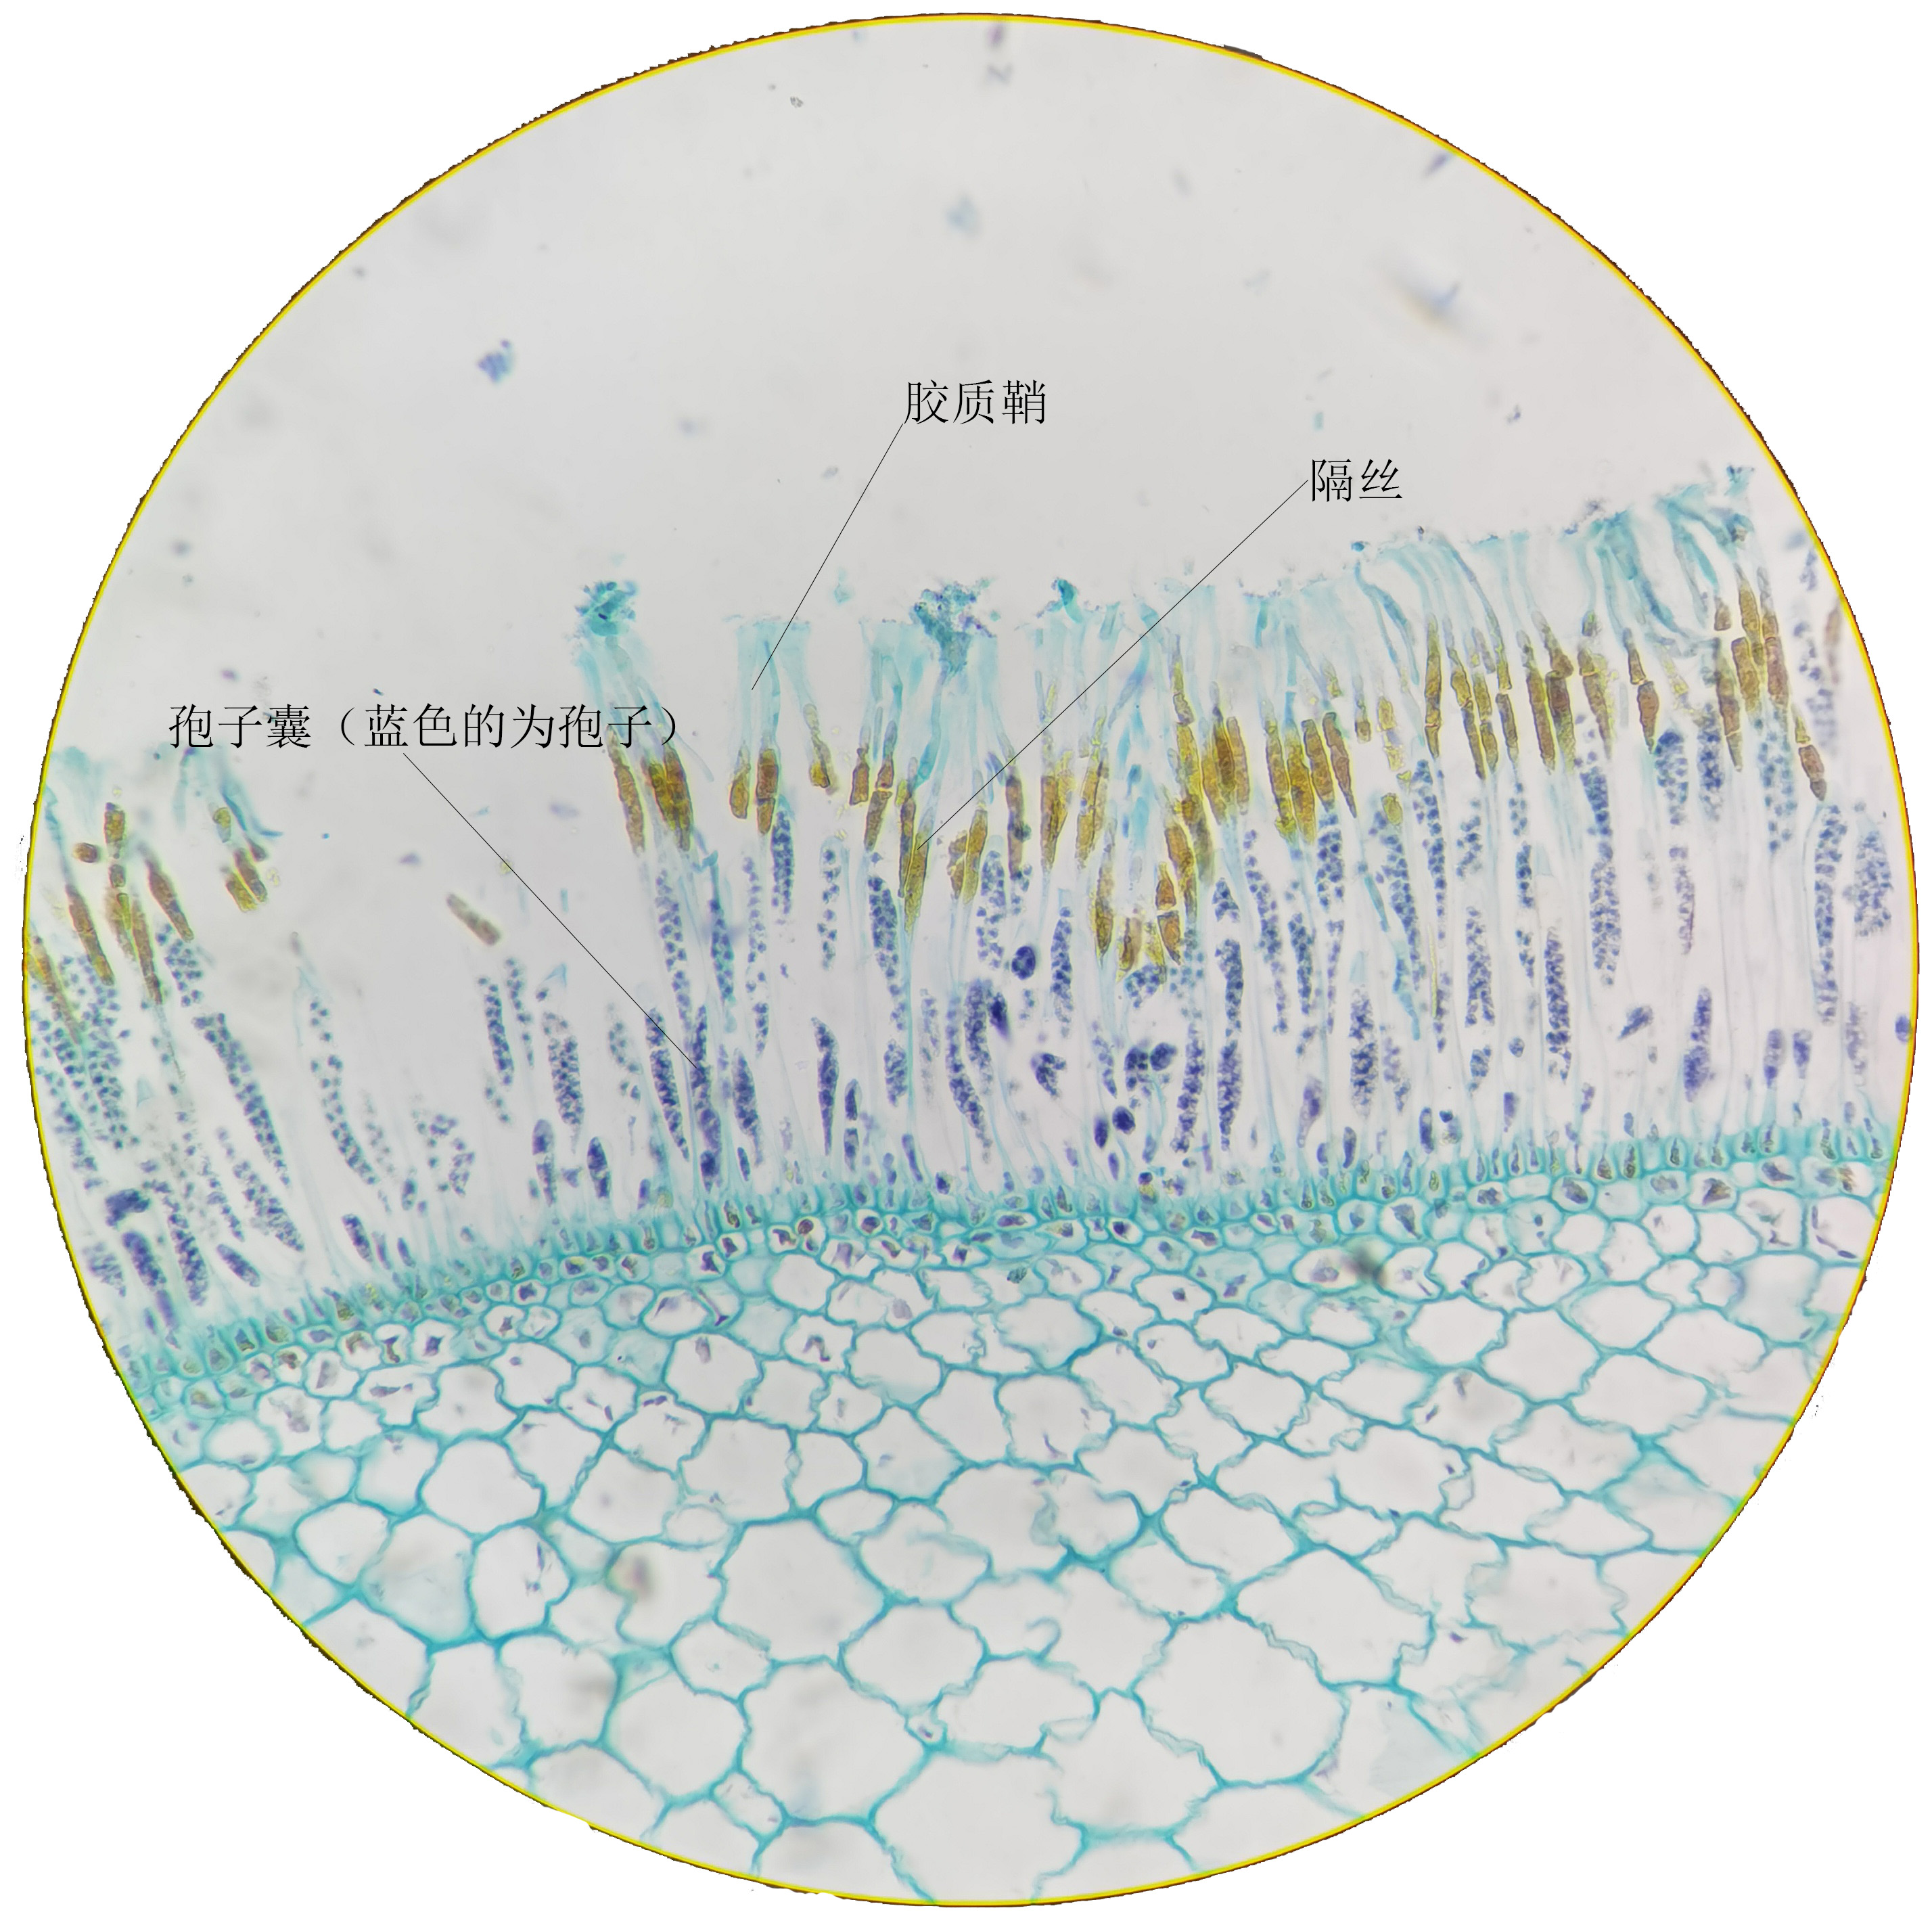
\includegraphics[scale = 0.08]{src/botany/IMG_20201118_192607.jpg}\label{haidai}}
                \subfigure[海带雌、 雄配子体]{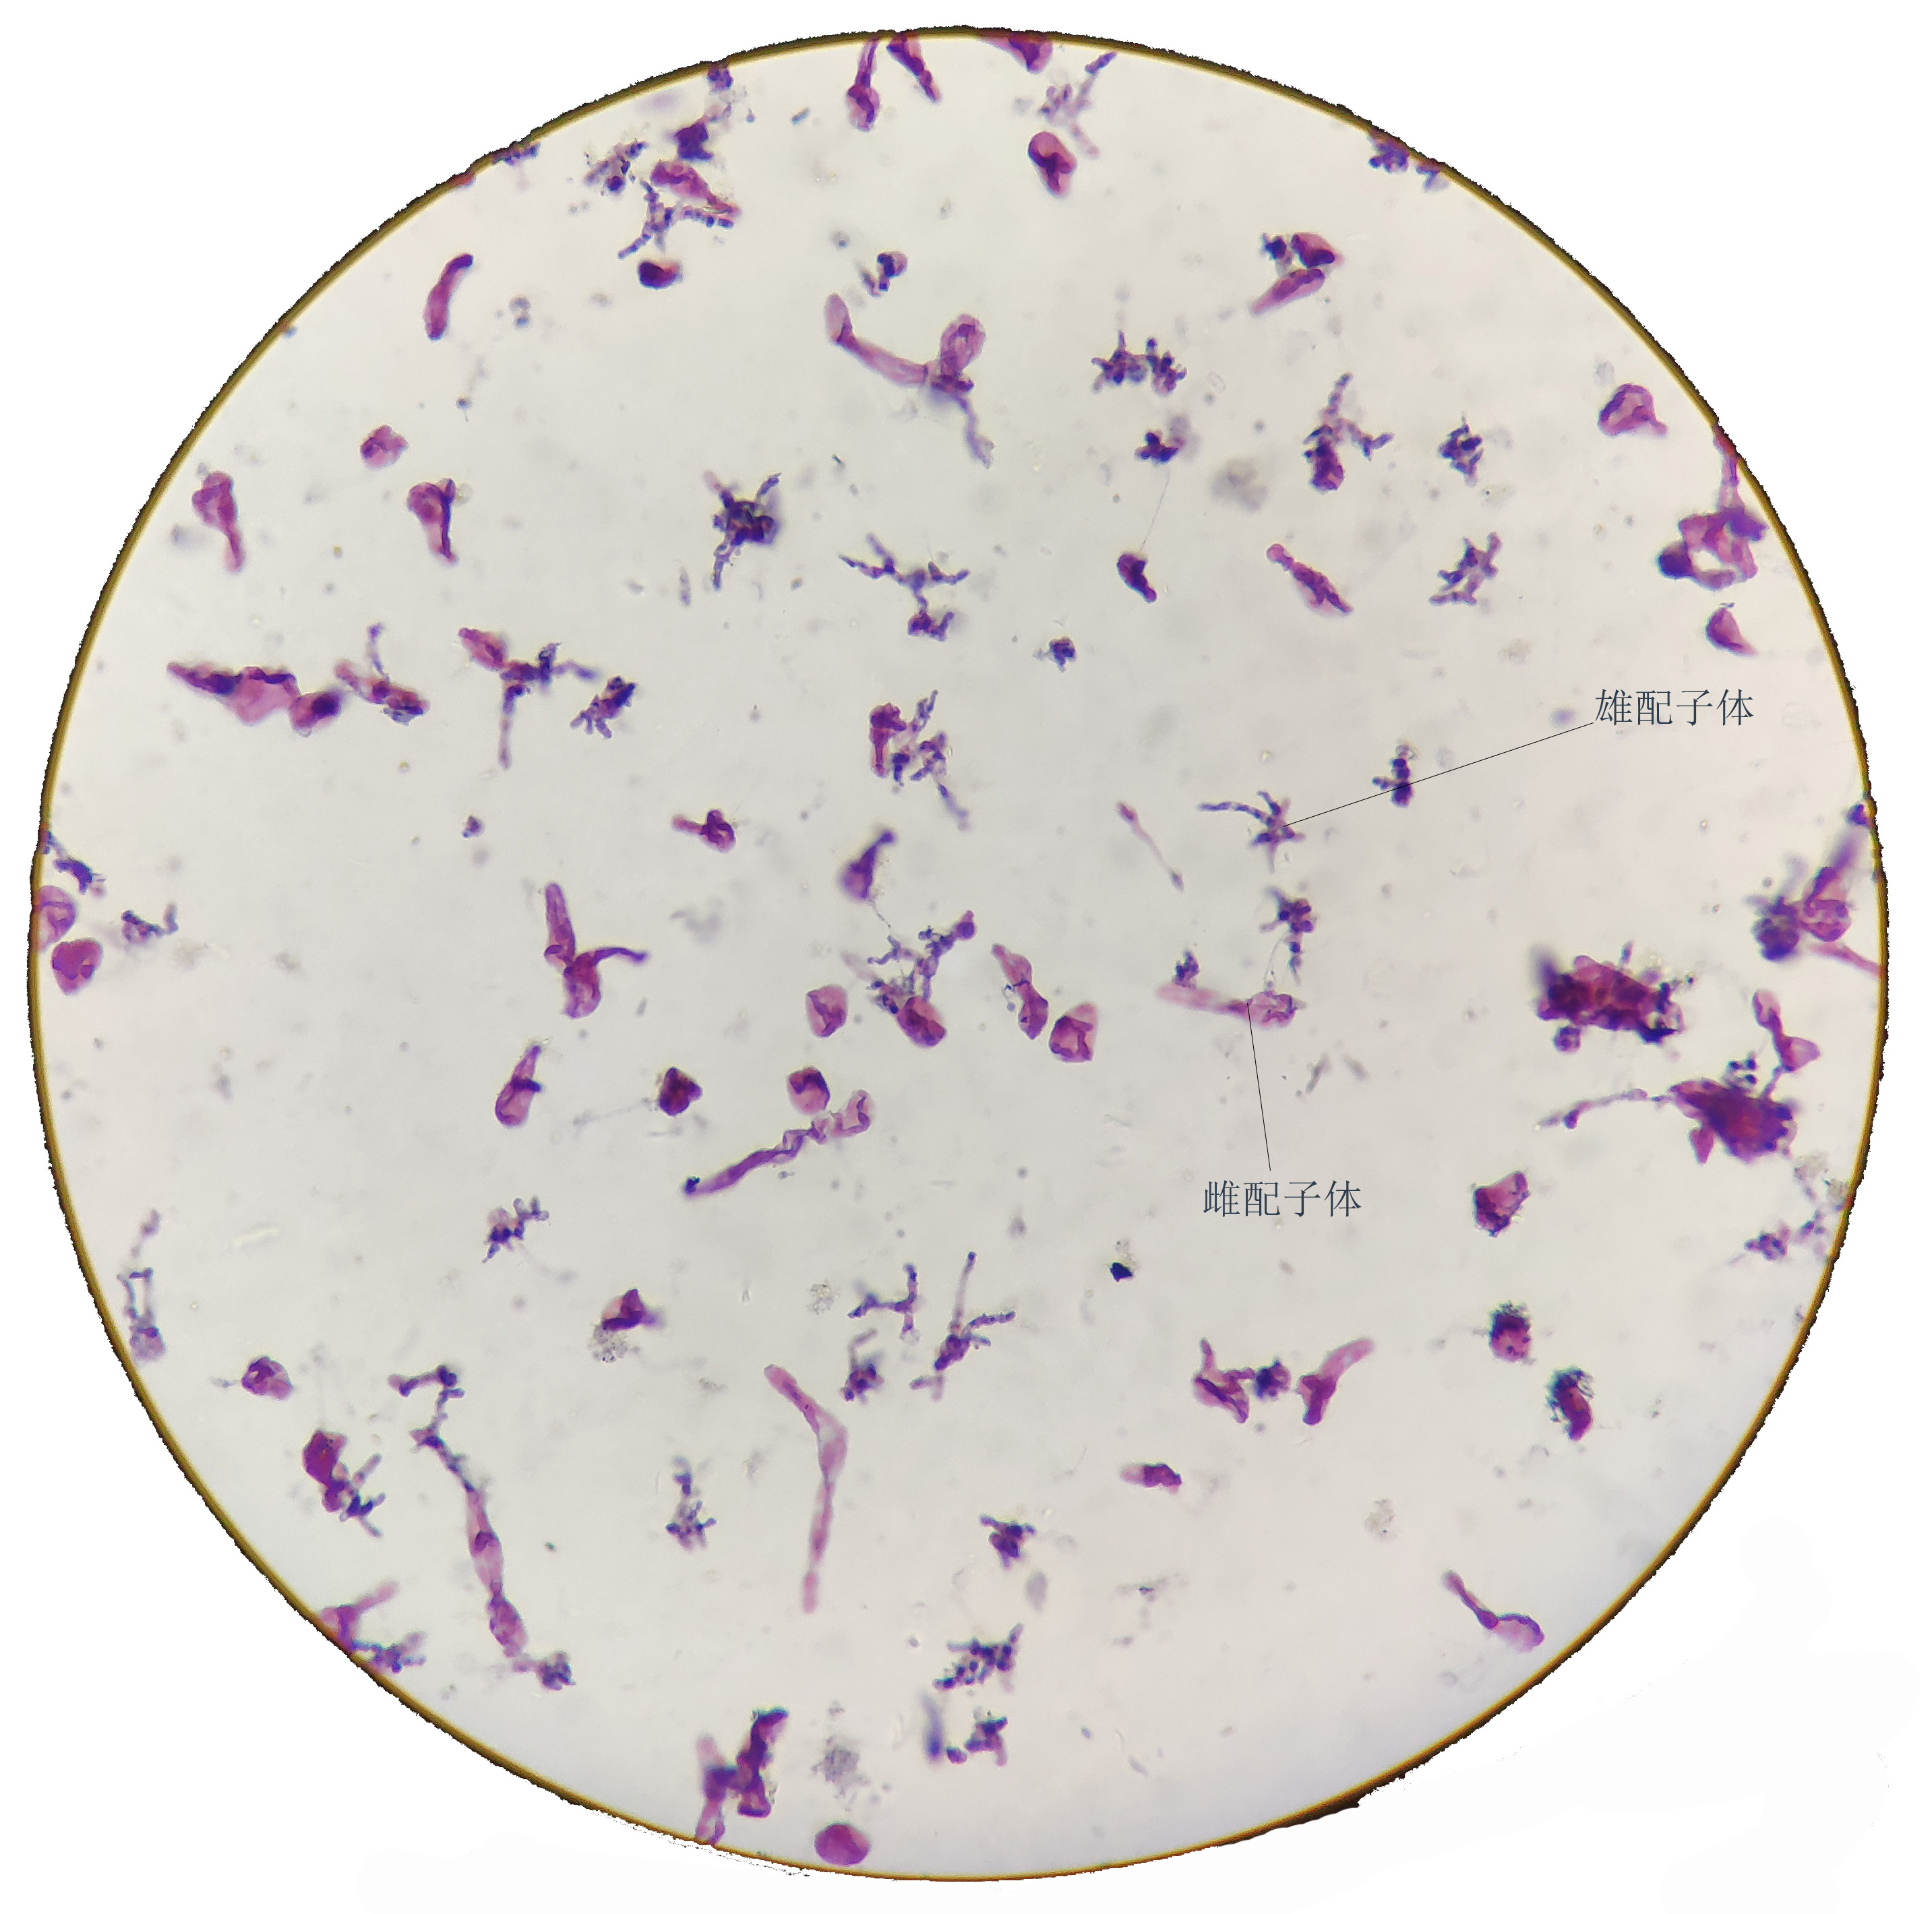
\includegraphics[scale=0.08]{src/botany/微信图片_20201217225710.jpg}\label{haidaipei}}
                \caption{实验一结果}
            \end{figure}
            \paragraph*{答:}见图\ref{shuimian}
            \paragraph*{2.用简图或照片显示水绵的有性生殖发生的方式和过程:}

            \paragraph*{3.用简图或照片显示海带带片细胞结构,重点显示孢子囊和孢子的形态}
                
            \paragraph*{答:}见图\ref{haidai}
            \paragraph*{4. 用简图或照片显示海带雌、 雄配子体的形态。}
            \paragraph*{答:}见图\ref{haidaipei}
        \subsection*{讨论}
            \paragraph*{1. 水绵生活史是否具有世代交替?为什么?}
            \paragraph*{答:}不存在。合子萌发时即减数分裂,无孢子体世代
            \paragraph*{2.海带的世代交替有什么特点?}
            \paragraph*{答:}属于孢子体占优势的异形世代交替
    \section{蘑菇的形态、结构与生殖}
        \subsection*{结果}
            \paragraph*{1.用简图或照片显示香菇子实层细胞结构以及担子、担孢子的形态;}
            \begin{figure}[h]
                \centering
                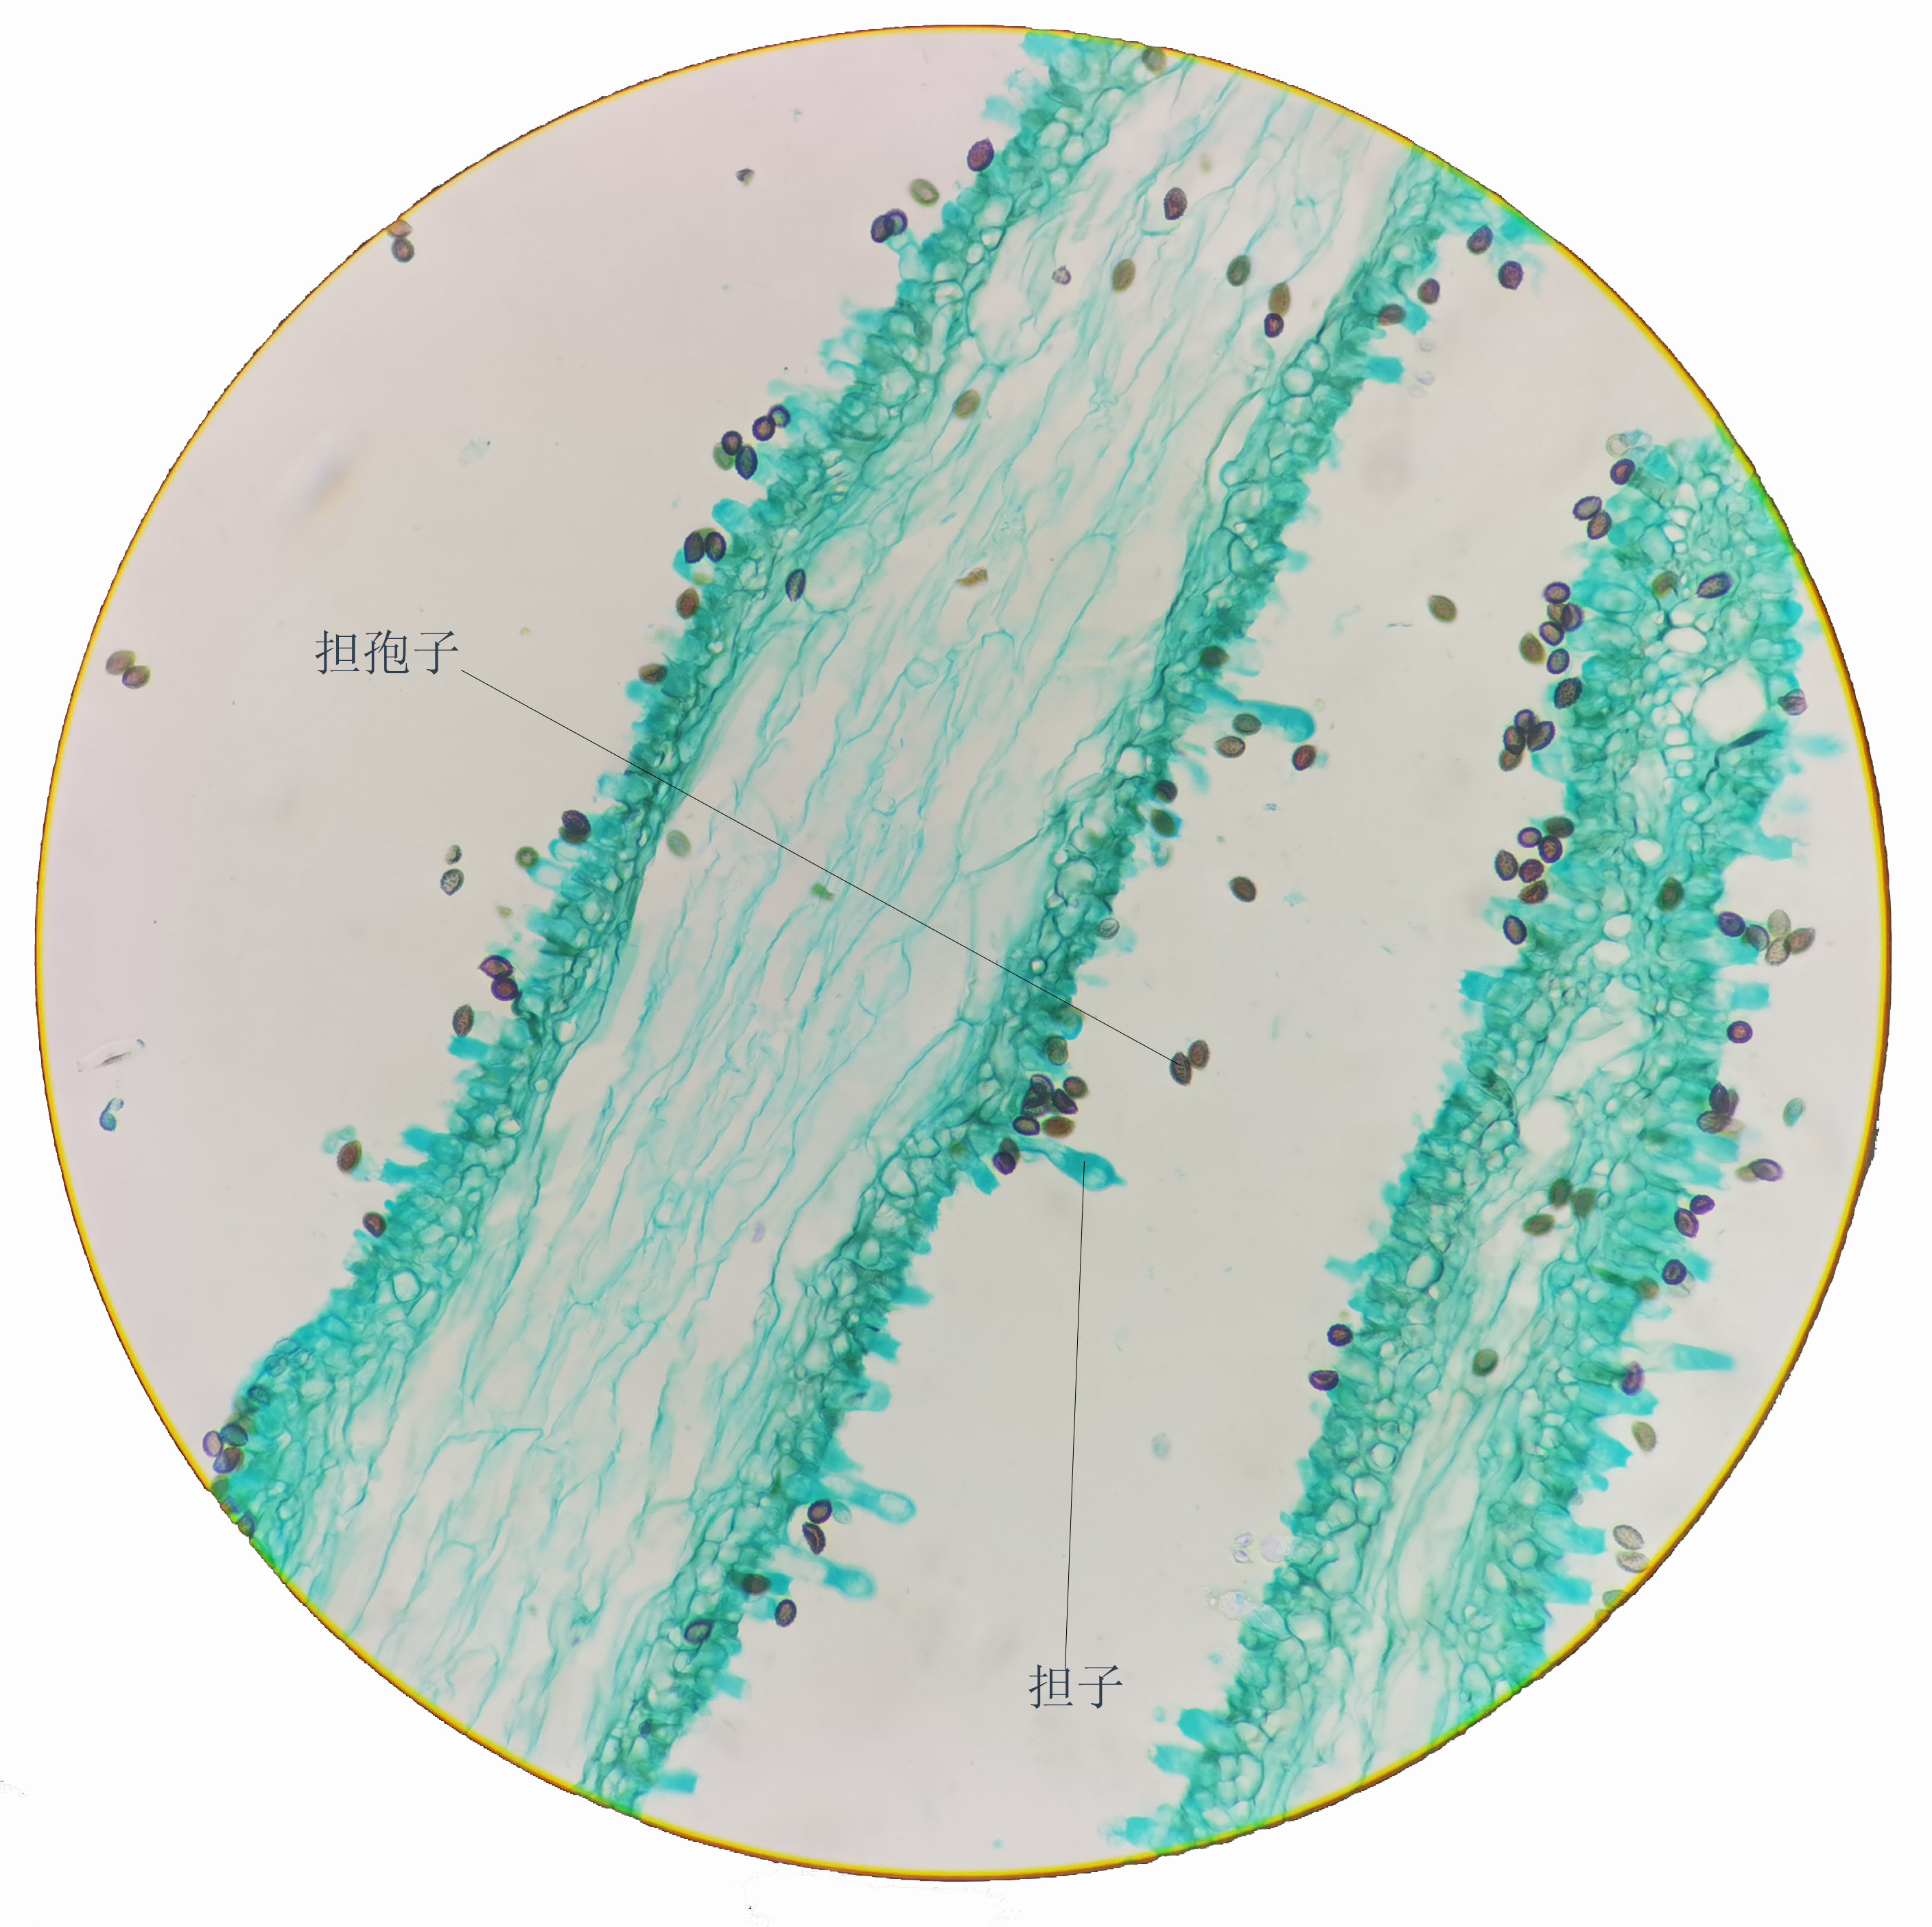
\includegraphics[scale=0.08]{src/botany/IMG_20201118_192210.jpg}
                \caption{香菇子实层细胞结构}
            \end{figure}
            \subsection*{讨论}
            \paragraph*{1.香菇的生活史具有什么特点?是否具有世代交替?}
            \paragraph*{答:}单倍体和二倍体均存在,产生锁状联合,存在世代交替
\end{document}